%!TEX TS-program = xelatex
%!TEX encoding = UTF-8 Unicode

\documentclass[tikz]{standalone}

\begin{document}
  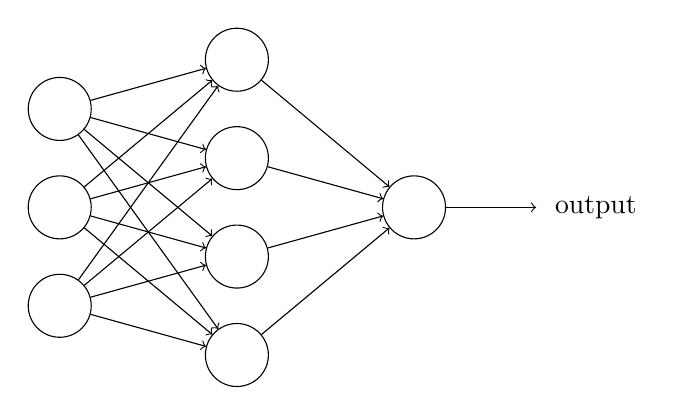
\begin{tikzpicture}[
    neuron/.style={circle,draw,inner sep=0pt,minimum size=8mm}
    ]

    % leftmost neutrons:
    \node (pl1) at (-2.25, 1.25) [neuron] {};
    \node (pl2) at (-2.25, 0) [neuron] {};
    \node (pl3) at (-2.25, -1.25) [neuron] {};

    % middle neutrons:
    \node (pm1) at (0, 1.875) [neuron] {};
    \node (pm2) at (0, 0.625) [neuron] {};
    \node (pm3) at (0, -0.625) [neuron] {};
    \node (pm4) at (0, -1.875) [neuron] {};

    % rightmost neutron:
    \node (pr) at (2.25, 0) [neuron] {};

    % output:
    \node (output) at (4.5, 0) {\ output};

    % connect nodes:

    \draw [->] (pl1) to (pm1);
    \draw [->] (pl1) to (pm2);
    \draw [->] (pl1) to (pm3);
    \draw [->] (pl1) to (pm4);
    \draw [->] (pl2) to (pm1);
    \draw [->] (pl2) to (pm2);
    \draw [->] (pl2) to (pm3);
    \draw [->] (pl2) to (pm4);
    \draw [->] (pl3) to (pm1);
    \draw [->] (pl3) to (pm2);
    \draw [->] (pl3) to (pm3);
    \draw [->] (pl3) to (pm4);
    \draw [->] (pm1) to (pr);
    \draw [->] (pm2) to (pr);
    \draw [->] (pm3) to (pr);
    \draw [->] (pm4) to (pr);
    \draw [->] (pr) to (output);

  \end{tikzpicture} 
\end{document}
